\documentclass[conference]{IEEEtran}
\IEEEoverridecommandlockouts
% The preceding line is only needed to identify funding in the first footnote. If that is unneeded, please comment it out.
\usepackage{cite}
\usepackage{amsmath,amssymb,amsfonts}
%\usepackage{algorithmic}
\usepackage{graphicx}
\usepackage{textcomp}
\usepackage{xcolor}

%\usepackage{algorithm}git add
\usepackage{algpseudocode}
\usepackage{arevmath}     % For math symbols

\usepackage[linesnumbered,ruled,vlined]{algorithm2e}
\newcommand\mycommfont[1]{\footnotesize\ttfamily\textcolor{blue}{#1}}
\SetCommentSty{mycommfont}
\SetKwInput{KwInput}{Input}                % Set the Input
\SetKwInput{KwOutput}{Output}              % set the Output

% Math font
%\usepackage{mathpazo}
\usepackage{fourier} 

% Enable subfigures
\graphicspath{ {./pictures/} }
\usepackage{subcaption}
\captionsetup{compatibility=false}

\def\BibTeX{{\rm B\kern-.05em{\sc i\kern-.025em b}\kern-.08em
    T\kern-.1667em\lower.7ex\hbox{E}\kern-.125emX}}
\begin{document}

\title{Analysis of Imbalanced Datasets\\
}

\author{\IEEEauthorblockN{Miguel Jiménez Aparicio}
\IEEEauthorblockA{
Atlanta, USA\\
maparicio6@gatech.edu}
\and
\IEEEauthorblockN{Belén Martín Urcelay}
\IEEEauthorblockA{
San Sebastián, Spain \\
burcelay3@gatech.edu}
\and
\IEEEauthorblockN{Cristian Gómez Peces}
\IEEEauthorblockA{
Atlanta, USA \\
cpeces3@gatech.edu}
}

\maketitle

\begin{abstract}
This document analyzes the impact of imbalanced datasets on machine learning classifiers. It discusses several techniques to deal with the imbalance. The results are applied to train a Twitter fake account detection algorithm where the performance of these techniques is compared. 
\end{abstract}

\begin{IEEEkeywords}
imbalance
\end{IEEEkeywords}

\section{Introduction}
	\subsection{Motivation}
	Many canonical machine learning algorithms used for classification assume that the number of objects in the respective classes is roughly the same. However, in reality, classes are rarely represented equally. In fact, class distribution skews are not only common, but many times expected \cite{data_imbalance_overview}, especially in decision systems aiming to detect rare but important cases. For instance, Covid-19 testing at Georgia Institute of Technology showed that less than 1\% of the samples contained the virus. This means that a naive classifier could achieve a 99\% accuracy just by labeling all samples as negative for Covid-19.
	
Imbalanced datasets significantly compromise the performance of many traditional learning algorithms. The disparity of classes in the training dataset may lead the algorithm to bias the classification towards the class with more instances, or even to ignore the minority class altogether. Therefore, it is vital to find efficient ways of dealing with data imbalances.

	The overall goal of our project is to provide an overview of the state-of-the-art approaches to solve the issues introduced by imbalanced datasets. Including, a performance comparison of the various techniques. We also aim to implement an efficient scheme that is able to deal with highly complex and imbalanced datasets.


	\subsection{Methodology}
	Firstly, we study a synthetic dataset characterized by its simplicity. It is made up of two classes following $N(\boldsymbol\mu_0, \Sigma_0)$ and $N(\boldsymbol\mu_1, \Sigma_1))$, where
			\begin{equation*}
				\boldsymbol\mu_0=
				\begin{pmatrix}
					-1\\
					-0.5
				\end{pmatrix},\ %\quad
				\boldsymbol\mu_1=
				\begin{pmatrix}
					0\\
					1
				\end{pmatrix},\ %\quad \\
				\Sigma_0=
				\begin{pmatrix}
					1 & 0\\
					0 & 1
				\end{pmatrix},\ %\quad %\mathrm{ and }\quad
				\Sigma_1=
				\begin{pmatrix}
					4 & 0\\
					0 & 2
				\end{pmatrix}
			\end{equation*} and where the minority class only accounts for 15\% of the samples. This simple dataset is especially useful to analyze the imbalance-compensating techniques from a mathematical perspective. Not only do we study the concepts learnt in class at a theoretical level, but we also use plugin machine learning models to illustrate how they affect density distributions.

		Secondly, we target a more complex dataset.  TODO

		The performance of the classification will be evaluated using the $F_1$ score $\in [0, 1]$, where the best possible score is 1. This metric is computed as
			\begin{equation*}
				F_1 = 2\frac{\mathrm{precision}\times\mathrm{recall}}{\mathrm{precision}+\mathrm{recall}},
			\end{equation*}
where the precision is the ratio between correctly identified minority samples and the total number of minority samples, while the recall is given by the fraction of correctly identified minority samples over all samples.

	\subsection{Accomplishments}


\section{Overview of the techniques}
	\subsection{Undersampling}
		Undersampling is frequently employed to balance datasets before any machine learning algorithm is applied. Undersampling involves randomly removing entries from the majority class. Figure \ref{fig:Undersampling_2D_OriginalHistograms} shows the effects of undersampling on the Gaussian training dataset. The class imbalance is somewhat countered. However, the algorithm learnt from this undersampled dataset will be affected. Namely, its ability to generalize and its posterior distribution.
			\begin{figure}
			     \centering
			     \begin{subfigure}[b]{0.24\textwidth}
			         \centering
			         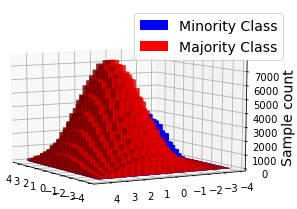
\includegraphics[width=\textwidth]{Undersampling_2D_OriginalDataset}
			         \caption{Original.}
			         \label{fig:Undersampling_2D_OriginalDataset}
			     \end{subfigure}
			     \hfill
			     \begin{subfigure}[b]{0.24\textwidth}
			         \centering
			         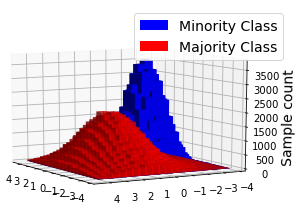
\includegraphics[width=\textwidth]{Undersampling_2D_UndersampledDataset}
			         \caption{Undersampled. $\beta=0.25$.}
			         \label{fig:Undersampling_2D_UndersampledDataset}
			     \end{subfigure}
			        \caption{Gaussian dataset.}
			        \label{fig:Undersampling_2D_OriginalHistograms}
			\end{figure}

	%\medskip
	\subsubsection{Generalization Ability}
		Induction algorithms require a sufficient amount of data to learn a model that generalizes well.  If the training set is not large, a classifier may just memorize the characteristics of the training data. Moreover, undersampling has the potential of eliminating valuable samples from consideration of the classifier entirely \cite{undersampling_generalization}, so it may exacerbate this problem of lack of data. The obtained training set may vary greatly from one undersampling to another, this leads to a high variance of the learned model. Hence, the achievable complexity of the hypothesis set must be reduced to ensure a good generalization.
		
	\subsubsection{Posterior Bias}
		One goal of undersampling is to change the priori probabilities of the classes to make them more balanced. The classifier assumes that the features it encounters at testing follow the same distribution as the training set. This mismatch introduced by design is known as sampling selection bias \cite{sampling_bias} on posterior distribution.

		Let $(\mathcal{X}, \mathcal{Y})$ denote the pairs of feature vectors, $\mathbf{x} \in \mathbb{R}^n$,  and binary labels, $y \in \{0, 1\}$, contained in our original dataset. We assume that the number of samples labeled as zero is small compared with the number of samples in class one. Undersampling randomly removes points from the majority class, we describe this sampling with the binary random variable $S$, which takes the value 1 if a sample is selected.

		It is reasonable to assume that the selection is independent of the features given the class. Then, applying Bayes rule, the law of total probability and noting that the samples from the minority class are always selected we obtain
		\begin{align*} \label{posterior}
			p' = & P(y=0|\mathbf{x}, s=1)=  \frac{P(s=1|y=0, \mathbf{x})P(y=0|\mathbf{x})}{P(s=1|\mathbf{x})}=\notag\\
					=&  \frac{P(y=0|\mathbf{x})}{P(y=0|\mathbf{x})+P(s=1|y=1)P(y=1|\mathbf{x})}=\notag\\
=&\frac{p}{p+\beta(1-p)},
		\end{align*}
where $p$ and $p'$ denote the posterior probability of encountering a sample from the minority class when employing the original and the undersampled dataset respectively. Whereas $\beta$ denotes the probability of keeping a sample from the majority class.

		The posterior is highly affected by the rate of the sampling. As more samples are removed, the classification is more biased towards the minority class. Figure \ref{fig.:Undersampling_2D_Contour_Classification} shows the decision region of a naive Bayes classifier. As the training set is undersampled the region of points that are labeled as the minority class grows. The rate of undersampling not only influences the posterior bias, but also the algorithm's ability to generalize. Thus, $\beta$ should be chosen with care. Figure \ref{fig.:Undersampling_F1_Score} presents the average F1-score over different training sets. We observe that the score is concave and in this case the optimum occurs with $\beta=0.82$.

			\begin{figure}
				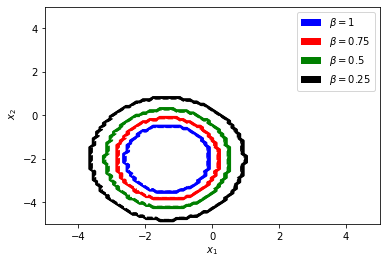
\includegraphics[scale=0.3]{Undersampling_2D_Contour_Classification}
				\centering
				\caption{Influence of undersampling on the classification region of a naive Bayes classifier trained with the Gaussian dataset. The area within each circle corresponds to the cluster of points that are classified as the minority class for a given undersampling rate.}
				\label{fig.:Undersampling_2D_Contour_Classification}
			\end{figure}
			\begin{figure}
				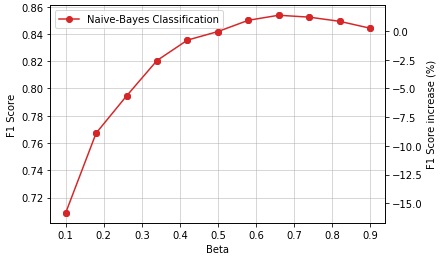
\includegraphics[scale=0.3]{Undersampling_F1_Score}
				\centering
				\caption{F1-score vs. undersampling rate.}
				\label{fig.:Undersampling_F1_Score}
			\end{figure}
		Another factor that strongly influences the posterior bias is class separability. The bias is higher when conditional distributions are similar across the classes\cite{undersampling_posterior}. To analyze this behaviour we reduced the problem to a one-dimensional setting, the results are depicted in Figure \ref{fig:Undersampling_posterior}. We confirm that undersampling shifts the posterior distribution in favor of the minority class. Nevertheless, the shift caused by $\beta$ is lower under the configuration with lower overlap.
			\begin{figure}
			     \centering
			     \begin{subfigure}[b]{0.24\textwidth}
			         \centering
			         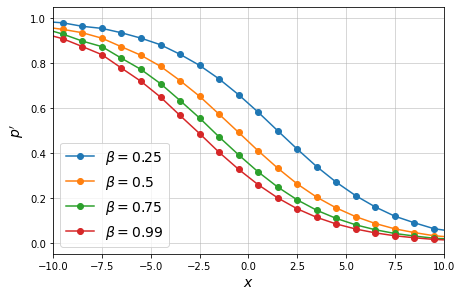
\includegraphics[width=\textwidth]{Undersampling_PosteriorBias}
			         \caption{$|\mu_0 - \mu_1|=3$.}
			         \label{fig:Undersampling_PosteriorBias}
			     \end{subfigure}
			     \hfill
			     \begin{subfigure}[b]{0.24\textwidth}
			         \centering
			         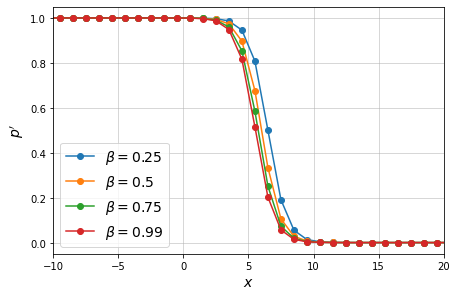
\includegraphics[width=\textwidth]{Undersampling_PosteriorBias_Separated}
			         \caption{$|\mu_0 - \mu_1|=13$.}
			         \label{fig:Undersampling_2D_UndersampledDataset}
			     \end{subfigure}
			        \caption{Influence of undersampling on posterior probability of the minority class.}
			        \label{fig:Undersampling_posterior}
			\end{figure}
		

	\subsection{Oversampling}

	\subsection{Cost-Sensitive Techniques}
	Blabla

\section{Classification impact on Real Data}
Ensemble of classifiers are known to improve the performance of single classifiers in imbalanced datasets [A Review on Ensembles for the Class Imbalance] by combining separate weak learners into a composite whole. Both bagging and boosting algorithms have been implemented from scratch to explore their advantages and compare them with highly-effective classifiers such as XGBoost. 

\subsection{Bagging}
Blabla

\break
\subsection{AdaBoost}
Unlike bagging, boosting fits the weak learners in an adaptive way: a different significance is assigned to each of the base learners based on the samples that were misclassified in the previous model. In particular, the AdaBoost algorithm stands out in the field of ensemble learning [Cost-sensitive boosting algorithms: Do we really need them?]. One its main advantages is the versatility to incorporate cost-sensitive techniques. We have implemented our a custom AdaBoost classifier to enables us to gain control over the algorithm at a lower level, make adjustments if necessary and create other Adaboost-based classifiers such as AdaCost or Boosted SVM. 

This custom implementation uses single decision trees with 2 leaf nodes and. It is given the number of maximum iterations (weak learners) that will be fitted, and a dataset $D$ formed by N training samples, each constituted by a feature vector $\boldsymbol{x}_i$ and a binary label $y_i$. For each iteration, we create the weak classifier based on the weighted training samples. For the first iteration, we allocate the same weight for all the samples ($1/N$). Once the simple decision trees has been created, we predict the class of every training sample and compute the weighted misclassification error $\epsilon_t$ for that decision tree. Its significance $\alpha_t$ is calculated based on that error and finally the weights of each training samples are updated depending on the signficance and whether the sample was correctly classified or not. Note that the weights are increased $e^{\alpha}$ times if the sample is misclassified or decreased by $e^{-\alpha}$ if correctly classified, with  $\alpha_t \in [0,1]$ because $\epsilon_t \in [0,0.5]$. The algorithm is fully detailed below.

\begin{algorithm}
  
  \KwInput{Training set $D = \{x_i, y_i\}, i=1,\dots,N;$ and $y_i \in \{ -1,+1\}$; $T:$ Number of iterations; $I:$ Weak learner} 
  \KwOutput{Boosted Classifier: $H(x)=sign\left( \sum^T_{t=1}\alpha_ih_t(x)\right)$ where $h_t, \alpha_t$ are the induced classifiers and their significance, respectively}
  %\KwData{Testing set $x$}
  $W_1(i) \leftarrow 1/N$ for $i=1,\dots,N$ %\tcp*{this is a comment}
  
  \tcc{Create a weak learner in each iteration}
  \For{t=1 to T}
    {
        $h_t \leftarrow I(D,W)$
        
        $\epsilon_t \leftarrow \sum^N_{i=1}W_t(i)[h_t(x_i)\neq y_i]$
        
        \If{$\epsilon_t > 0.5$}
        		{
		
		$T \leftarrow t-1$
		
		\bf{return}
		}
		
	$\alpha_t = \frac{1}{2}\ln \left( \frac{1-\epsilon_t}{\epsilon_t} \right)$
	
	\tcc{Update Weights}
	  
	 $W_{t+1}(i) = W_t(i) e^{(-\alpha_th_t(x_i)y_i)}$ for $i=1,\dots,N$
	 
	 Normalize $W_{t+1}$ such that $\sum^N_{i=1}W_{t+1}(i)=1$
	  
    }


\caption{AdaBoost Algorithm}
\end{algorithm}


---- Mathematical implications ----




\subsection{AdaCost}
Blabla

\subsection{Boosting SVM}

\begin{algorithm}
  
 \KwInput{Training set $D = \{x_i, y_i\}, i=1,\dots,N;$ and $y_i \in \{ -1,+1\}$; $T:$ Maximum number of iterations; The initial $\sigma=\sigma_{ini}, \sigma_{min}, \sigma_{step}$} 
\KwOutput{Boosted Classifier: $H(x)=sign\left( \sum^T_{t=1}\alpha_ih_t(x)\right)$ where $h_t, \alpha_t$ are the induced classifiers and their significance, respectively}
  %\KwData{Testing set $x$}
  $W_1(i) \leftarrow 1/N$ for $i=1,\dots,N$ %\tcp*{this is a comment}
  
  \tcc{Create a weak learner in each iteration}
  \While{$\sigma > \sigma_{min}$ and $t<T$}
    {
        $t \leftarrow t+1$
        
        $h_t \leftarrow RBFSVM(D,W,\sigma)$ \tcp*{Train RBFSVM}
        
        $\epsilon_t \leftarrow \sum^N_{i=1}W_t(i)[h_t(x_i)\neq y_i]$
        
        \If{$\epsilon_t > 0.5$}
        		{
		
		$\sigma \leftarrow \sigma - \sigma_{step}$
		
		}
	\Else
	{
	$\alpha_t = \frac{1}{2}\ln \left( \frac{1-\epsilon_t}{\epsilon_t} \right)$
	
	\tcc{Update Weights}
	  
	 $W_{t+1}(i) = W_t(i) e^{(-\alpha_th_t(x_i)y_i)}$ for $i=1,\dots,N$
	 
	 Normalize $W_{t+1}$ such that $\sum^N_{i=1}W_{t+1}(i)=1$
	 }
    }
\caption{Boosted SVM Algorithm}
\end{algorithm}

\subsection{AdaMEC}
Blabla

\subsection{XGBoost}
Blabla

\section{Results and Discussion}
Finally, we have combined them with downsampling to explore the effectiveness of hybrid algorithms.
Blabla 

\section{Conclusions}
Blabla 

\break
\subsection{Abbreviations and Acronyms}\label{AA}
Define abbreviations and acronyms the first time they are used in the text, 
even after they have been defined in the abstract. Abbreviations such as 
IEEE, SI, MKS, CGS, ac, dc, and rms do not have to be defined. Do not use 
abbreviations in the title or heads unless they are unavoidable.

\subsection{Units}
\begin{itemize}
\item Use either SI (MKS) or CGS as primary units. (SI units are encouraged.) English units may be used as secondary units (in parentheses). An exception would be the use of English units as identifiers in trade, such as ``3.5-inch disk drive''.
\item Avoid combining SI and CGS units, such as current in amperes and magnetic field in oersteds. This often leads to confusion because equations do not balance dimensionally. If you must use mixed units, clearly state the units for each quantity that you use in an equation.
\item Do not mix complete spellings and abbreviations of units: ``Wb/m\textsuperscript{2}'' or ``webers per square meter'', not ``webers/m\textsuperscript{2}''. Spell out units when they appear in text: ``. . . a few henries'', not ``. . . a few H''.
\item Use a zero before decimal points: ``0.25'', not ``.25''. Use ``cm\textsuperscript{3}'', not ``cc''.)
\end{itemize}

\subsection{Equations}
Number equations consecutively. To make your 
equations more compact, you may use the solidus (~/~), the exp function, or 
appropriate exponents. Italicize Roman symbols for quantities and variables, 
but not Greek symbols. Use a long dash rather than a hyphen for a minus 
sign. Punctuate equations with commas or periods when they are part of a 
sentence, as in:
\begin{equation}
a+b=\gamma\label{eq}
\end{equation}

Be sure that the 
symbols in your equation have been defined before or immediately following 
the equation. Use ``\eqref{eq}'', not ``Eq.~\eqref{eq}'' or ``equation \eqref{eq}'', except at 
the beginning of a sentence: ``Equation \eqref{eq} is . . .''

\subsection{\LaTeX-Specific Advice}

Please use ``soft'' (e.g., \verb|\eqref{Eq}|) cross references instead
of ``hard'' references (e.g., \verb|(1)|). That will make it possible
to combine sections, add equations, or change the order of figures or
citations without having to go through the file line by line.

Please don't use the \verb|{eqnarray}| equation environment. Use
\verb|{align}| or \verb|{IEEEeqnarray}| instead. The \verb|{eqnarray}|
environment leaves unsightly spaces around relation symbols.

Please note that the \verb|{subequations}| environment in {\LaTeX}
will increment the main equation counter even when there are no
equation numbers displayed. If you forget that, you might write an
article in which the equation numbers skip from (17) to (20), causing
the copy editors to wonder if you've discovered a new method of
counting.

{\BibTeX} does not work by magic. It doesn't get the bibliographic
data from thin air but from .bib files. If you use {\BibTeX} to produce a
bibliography you must send the .bib files. 

{\LaTeX} can't read your mind. If you assign the same label to a
subsubsection and a table, you might find that Table I has been cross
referenced as Table IV-B3. 

{\LaTeX} does not have precognitive abilities. If you put a
\verb|\label| command before the command that updates the counter it's
supposed to be using, the label will pick up the last counter to be
cross referenced instead. In particular, a \verb|\label| command
should not go before the caption of a figure or a table.

Do not use \verb|\nonumber| inside the \verb|{array}| environment. It
will not stop equation numbers inside \verb|{array}| (there won't be
any anyway) and it might stop a wanted equation number in the
surrounding equation.

\subsection{Some Common Mistakes}\label{SCM}
\begin{itemize}
\item The word ``data'' is plural, not singular.
\item The subscript for the permeability of vacuum $\mu_{0}$, and other common scientific constants, is zero with subscript formatting, not a lowercase letter ``o''.
\item In American English, commas, semicolons, periods, question and exclamation marks are located within quotation marks only when a complete thought or name is cited, such as a title or full quotation. When quotation marks are used, instead of a bold or italic typeface, to highlight a word or phrase, punctuation should appear outside of the quotation marks. A parenthetical phrase or statement at the end of a sentence is punctuated outside of the closing parenthesis (like this). (A parenthetical sentence is punctuated within the parentheses.)
\item A graph within a graph is an ``inset'', not an ``insert''. The word alternatively is preferred to the word ``alternately'' (unless you really mean something that alternates).
\item Do not use the word ``essentially'' to mean ``approximately'' or ``effectively''.
\item In your paper title, if the words ``that uses'' can accurately replace the word ``using'', capitalize the ``u''; if not, keep using lower-cased.
\item Be aware of the different meanings of the homophones ``affect'' and ``effect'', ``complement'' and ``compliment'', ``discreet'' and ``discrete'', ``principal'' and ``principle''.
\item Do not confuse ``imply'' and ``infer''.
\item The prefix ``non'' is not a word; it should be joined to the word it modifies, usually without a hyphen.
\item There is no period after the ``et'' in the Latin abbreviation ``et al.''.
\item The abbreviation ``i.e.'' means ``that is'', and the abbreviation ``e.g.'' means ``for example''.
\end{itemize}
An excellent style manual for science writers is \cite{b7}.

\subsection{Authors and Affiliations}
\textbf{The class file is designed for, but not limited to, six authors.} A 
minimum of one author is required for all conference articles. Author names 
should be listed starting from left to right and then moving down to the 
next line. This is the author sequence that will be used in future citations 
and by indexing services. Names should not be listed in columns nor group by 
affiliation. Please keep your affiliations as succinct as possible (for 
example, do not differentiate among departments of the same organization).

\subsection{Identify the Headings}
Headings, or heads, are organizational devices that guide the reader through 
your paper. There are two types: component heads and text heads.

Component heads identify the different components of your paper and are not 
topically subordinate to each other. Examples include Acknowledgments and 
References and, for these, the correct style to use is ``Heading 5''. Use 
``figure caption'' for your Figure captions, and ``table head'' for your 
table title. Run-in heads, such as ``Abstract'', will require you to apply a 
style (in this case, italic) in addition to the style provided by the drop 
down menu to differentiate the head from the text.

Text heads organize the topics on a relational, hierarchical basis. For 
example, the paper title is the primary text head because all subsequent 
material relates and elaborates on this one topic. If there are two or more 
sub-topics, the next level head (uppercase Roman numerals) should be used 
and, conversely, if there are not at least two sub-topics, then no subheads 
should be introduced.

\subsection{Figures and Tables}
\paragraph{Positioning Figures and Tables} Place figures and tables at the top and 
bottom of columns. Avoid placing them in the middle of columns. Large 
figures and tables may span across both columns. Figure captions should be 
below the figures; table heads should appear above the tables. Insert 
figures and tables after they are cited in the text. Use the abbreviation 
``Fig.~\ref{fig}'', even at the beginning of a sentence.

\begin{table}[htbp]
\caption{Table Type Styles}
\begin{center}
\begin{tabular}{|c|c|c|c|}
\hline
\textbf{Table}&\multicolumn{3}{|c|}{\textbf{Table Column Head}} \\
\cline{2-4} 
\textbf{Head} & \textbf{\textit{Table column subhead}}& \textbf{\textit{Subhead}}& \textbf{\textit{Subhead}} \\
\hline
copy& More table copy$^{\mathrm{a}}$& &  \\
\hline
\multicolumn{4}{l}{$^{\mathrm{a}}$Sample of a Table footnote.}
\end{tabular}
\label{tab1}
\end{center}
\end{table}

\begin{figure}[htbp]
\centerline{
\includegraphics{pictures/fig1.png}}
\caption{Example of a figure caption.}
\label{fig}
\end{figure}

Figure Labels: Use 8 point Times New Roman for Figure labels. Use words 
rather than symbols or abbreviations when writing Figure axis labels to 
avoid confusing the reader. As an example, write the quantity 
``Magnetization'', or ``Magnetization, M'', not just ``M''. If including 
units in the label, present them within parentheses. Do not label axes only 
with units. In the example, write ``Magnetization (A/m)'' or ``Magnetization 
\{A[m(1)]\}'', not just ``A/m''. Do not label axes with a ratio of 
quantities and units. For example, write ``Temperature (K)'', not 
``Temperature/K''.

\section*{Acknowledgment}

The preferred spelling of the word ``acknowledgment'' in America is without 
an ``e'' after the ``g''. Avoid the stilted expression ``one of us (R. B. 
G.) thanks $\ldots$''. Instead, try ``R. B. G. thanks$\ldots$''. Put sponsor 
acknowledgments in the unnumbered footnote on the first page.

\vspace{12pt}

\bibliographystyle{ieeetr} \bibliography{ECE6254_references}
\end{document}
